\documentclass[12pt]{article}
\usepackage[utf8]{inputenc}
\usepackage[czech]{babel}

\usepackage{graphicx}
\usepackage{placeins}
\usepackage[left=2cm, right=2cm,top=3cm, bottom=2cm]{geometry}
\usepackage{hyperref} 

\graphicspath{ {./} }

\begin{document}
\begin{titlepage}
   \begin{center}
        {\large Fakulta~aplikovaných věd Západočeské univerzity v~Plzni}
        \vspace{1cm}
        
\includegraphics{zcu-logo.png}
         \vspace{1.5cm}\par
        {\Huge
       \textbf{Dokumentace semestrální práce předmětu KIV/UPS}
		\par}
		\vfill
       \vspace{0.8cm}
      \begin{minipage}{0.4\textwidth}
            \begin{flushleft}
                \large
                Plzeň, \today
                
            \end{flushleft}
        \end{minipage}
        ~
        \begin{minipage}{0.4\textwidth}
            \begin{flushright}
               Karel Matějovský
            \end{flushright}
        \end{minipage}
            
   \end{center}
\end{titlepage}

\tableofcontents
\newpage
\section{Úvod}
Obsahem této semestrální práce je vytvoření programů serveru a klienta hry Blackjack. Semestrální práce má za úkol seznámit se se základy komunikace v síti a technologiemi použitými pro přenos dat

\newpage

\section{Popis průběhu hry}
Cílem blackjacku je mít takovou kombinaci vyšší než krupiérův, ale zároveň ne vyšší než 21. Pokud je váš součet vyšší než 21, je to "bust", což znamená, že jste vypadli ze hry.
Hru začínají všichni kromě krupiéra uzavřenímí sázky. Poté krupiér rozdá každému 2 karty.
Karty 2 až 10 se hodnotí pomocí jejich bodů.
Hodnota karty se počítá podle jejího líce, přičemž spodky, dámy a králové se všechny rovnají 10, esa mají hodnotu 1. Pokud jsou vaše dvě karty v součtu 21, vyhráváte jeden a půl násobek své sázky a pro toto kolo končíte.
V opačném případě se vás krupiér zeptá, zda chcete.
další kartu z horní části balíčku. Pokud ano, zvolíte "hit". Počet karet, které můžete mít, není omezen, ale jakmile váš součet karet v ruce překročí hranici 21, jste vyřazeni a krupiér dostane vaši sázku.
Pokud už žádné další karty nechcete, zvolíte "stay". Jakmile krupiér obejde stůl, pokud má hodnotu svých karet 16 nebo méně, musí si vzít další kartu. Pokud je na ní 17 nebo více, musí zůstat. Pokud krupiér překročí hodnotu 21, každý hráč, který je ještě v tomto kole, vyhrává dvojnásobek své sázky. Pokud však krupiér hranici nepřekročí, vyhrávají pouze.
hráči, jejichž kombinace jsou vyšší než hodnota karet krupiéra - vyhrávají dvojnásobek své sázky. Všichni ostatní svou původní sázku prohrají. Jakmile kolo skončí, všichni hráči
vsadí novou sázku a začíná další kolo.


\newpage
\section{Protokol}
\subsection{Formát zpráv}
Veškeré přenášené zprávy mají délku 24 bytů. Zpráva se dělí na tři části, každá o délce 8 bytů. První část 'Type' obsahuje typ zprávy, druhá a třetí část obsahují parametry zprávy. Pokud daná zpráva parametry neobsahuje, zůstávají prázdné. Aby bylo zabráněno chybám při obsahu částí kratší než 8 bytů, jsou veškeré prázdné části zprávy doplněny napravo od hodnoty dané části. Je-li např. v první části obsažena zpráva 'WIN', doplní se zbylé místo části mezerami tak, aby část obsahovala 'WIN␣␣␣␣␣'
\begin{figure}[htbp]
\centering
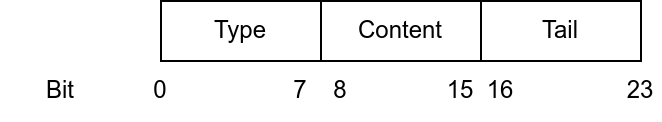
\includegraphics[width=0.5\textwidth]{protocol_structure.png}
\caption{Struktura zprávy protokolu}
\end{figure}

\subsection{Přenášené datové struktury, typy}
Zprávy jsou přenášeny jako řetězec znaků. Tyto znaky jsou dále interpretovány podle typu zprávy. Typ zprávy je vždy řetězec. Pokud je přenášen jiný datový typ než je řetězec, je převeden na řetězec a po přijetí převeden zpět. Toto se týká převážně číselných údajů.

\subsection{Význam přenášených dat a kódů}
Význam, směr a parametry přenášených kódů se nacházejí na následující stránce.

\begin{table}[]
\begin{tabular}{|l|l|l|p{5.5cm}|p{3cm}|}
\hline
\textbf{Odesílatel} & \textbf{Příkaz} & \textbf{Paramet}r        & \textbf{Očekáváná odpověď} & \textbf{Očekáváná odpověď                                                       } \\ \hline
C          & CONN            &                 & OK                                                                & Navázání spojení se serverem                        \\ \hline
C          & SENDNCKN        & Přezdívka hráče & LADDROOM \textless{}čísla~ místností\textgreater{}                  & Zaslání přezdívky hráče                             \\ \hline
S          & SETLBY          &                 & OK                                                                & Přepnutí pohledu na lobby                           \\ \hline
S          & SETGAME         &                 & OK                                                                & Přepnutí pohledu na hru                             \\ \hline
S          & LADDROOM        & Číslo místnosti & OK                                                                & Přidání místnosti do lobby                          \\ \hline
C          & JOINROOM        & Číslo místnosti & OK                                                                & Připojení se do místnosti                           \\ \hline
C          & GAMERDY         &                 & SHBETUI                                                           & Klient je připraven ke hře                          \\ \hline
S          & PLRRDY          & Přezdívka hráče & OK                                                                & Zpráva o připraveném klientovi ostatním             \\ \hline
S          & PLRNRDY         & Přezdívka hráče & OK                                                                & Zpráva o nepřipraveném klientovi ostatním           \\ \hline
C          & PLACEBET        & Hodnota sázky   & UPDBET,~CLRCARDS, 2x~DEALCARD                \textless{}názvy~karet\textgreater{} & Položení sázky                                      \\ \hline
S          & UPDCRDT         & Hodnota kreditu & OK                                                                & Aktualizace kreditu klienta                         \\ \hline
S          & UPDBET          & Hodnota sázky   & OK                                                                & Aktualizace sázky klienta                           \\ \hline
S          & CLRCARDS        &                 & OK                                                                & Ostranění viditelných karet klienta                 \\ \hline
S          & DEALCARD        & Název karty     & YOUTURN  nebo PLRTURNS                                            & Přidání karty klientovi                             \\ \hline
S          & PAUSE           &                 & OK                                                                & Pozastavení hry                                     \\ \hline
S          & UNPAUSE         &                 & OK                                                                & Zotavení hry                                        \\ \hline
C          & HIT             &                 & OK                                                                & Akce "hit"                                          \\ \hline
C          & STAY            &                 & OK                                                                & Akce "stay"                                         \\ \hline
\end{tabular}
\end{table}

\begin{table}[]
\begin{tabular}{|l|l|l|p{5.5cm}|p{3cm}|}
\hline
\textbf{Odesílatel} & \textbf{Příkaz} & \textbf{Paramet}r        & \textbf{Očekáváná odpověď} & \textbf{Očekáváná odpověď                                                            } \\ \hline
S          & LBYBTN          &                 & OK                                                                & Zobrazení tlačítka pro návrat do lobby              \\ \hline
C          & LEAVE           &                 & OK                                                                & Zobrazení tlačítka pro opuštění hry                 \\ \hline
S          & SHBTNRDY        &                 & GAMERDY                                                           & Zobrazení tlačítka pro potvrzení připraveného hráče \\ \hline
S          & SHBETUI         &                 & PLACEBET                                                          & Zobrazení nabídky sázení                            \\ \hline
S          & BUST            &                 & OK                                                                & Zpráva o události "bust"                            \\ \hline
S          & WIN             &                 & OK                                                                & Zpráva o výhře                                      \\ \hline
S          & LOSE            &                 & OK                                                                & Zpráva o prohře                                     \\ \hline
S          & HGRDLR          &                 & OK                                                                & Zpráva o částce vyšší než dealerově                 \\ \hline
S          & DLRBUSTS        &                 & OK                                                                & Zpráva o dealerově přesažení hraniční hodnoty karet \\ \hline
S          & YOUTURN         &                 & HIT / STAY                                                        & Zpráva, že je daný hráč na tahu                     \\ \hline
S          & PLRTURNS        & Přezdívka hráče & OK                                                                & Zpráva, že je jiný hráč na tahu                     \\ \hline
S          & PLRDSCN         & Přezdívka hráče & OK                                                                & Zpráva o odpojení jiného hráče                      \\ \hline
S          & PLRRCN          & Přezdívka hráče & OK                                                                & Zpráva o znovupřipojení jiného hráče                \\ \hline
S/C        & OK              &                 &                                                                   & Odpoveď na zaslanou validní zprávu                  \\ \hline
\end{tabular}
\end{table}

\newpage
\subsection{Omezení vstupních hodnot a validace dat}
Omezení vstupních hodnot se zde vyskytuje jen zřídka, jelikož se hra skládá především z jednoduchých tahů. Jsou však ošetřeny vstupy jako nevalidní číslo místnosti nebo sázení moc velké nebo naopak záporné částky. Je validován i převod z řetězce na čísla v případech, kdy je to zapotřebí. 

\subsection{Návaznost zpráv}
Ošetření návaznosti zpráv probíhá pomocí stavového diagramu. Hráči jsou stavy měněny za pomocí funkce 'changeState', která v závislosti na zadané tabulce vyhodnotí, zda-li je daný tah validní. Veškeré možné stavy klientů jsou uvedeny v následující tabulce

\begin{table}[htb]
\begin{tabular}{|l|}
\hline
INACTIVE                  \\ \hline
CONNECTING                \\ \hline
CONNECTED                 \\ \hline
LOBBY                     \\ \hline
GAME\_NOT\_READY          \\ \hline
GAME\_READY               \\ \hline
GAME\_PLACED\_BET         \\ \hline
GAME\_WAITING             \\ \hline
GAME\_TURN                \\ \hline
GAME\_WAITING\_NEW\_ROUND \\ \hline
GAME\_WAITING\_END        \\ \hline
\end{tabular}
\end{table}

Tabulka programu s přechody jednotlivých stavů vypadá následovně:

\begin{table}[!hbtp]
\begin{tabular}{|l|l|l|l|l|l|l|l|l|l|l|}
\hline
1 & 1 & 0 & 0 & 0 & 0 & 0 & 0 & 0 & 0 & 0 \\ \hline
1 & 1 & 1 & 0 & 0 & 0 & 0 & 0 & 0 & 0 & 0 \\ \hline
1 & 0 & 1 & 1 & 0 & 0 & 0 & 0 & 0 & 0 & 0 \\ \hline
1 & 0 & 0 & 1 & 1 & 0 & 0 & 0 & 0 & 0 & 0 \\ \hline
1 & 0 & 0 & 0 & 1 & 1 & 0 & 0 & 0 & 0 & 0 \\ \hline
1 & 0 & 0 & 0 & 0 & 1 & 1 & 0 & 0 & 0 & 0 \\ \hline
1 & 0 & 0 & 0 & 0 & 0 & 0 & 1 & 1 & 0 & 0 \\ \hline
1 & 0 & 0 & 0 & 0 & 0 & 0 & 1 & 1 & 0 & 0 \\ \hline
1 & 0 & 0 & 0 & 0 & 0 & 0 & 1 & 1 & 1 & 1 \\ \hline
1 & 0 & 0 & 0 & 0 & 1 & 0 & 1 & 1 & 1 & 0 \\ \hline
1 & 0 & 0 & 1 & 0 & 1 & 0 & 0 & 0 & 0 & 1 \\ \hline
\end{tabular}
\end{table}
\newpage
Následující obrázek ilustruje přechody stavového diagramu klienta. Přechody ze všech stavů do stavu INACTIVE nejsou zakresleny kvůli přehlednosti.

\begin{figure}[htbp]
\centering
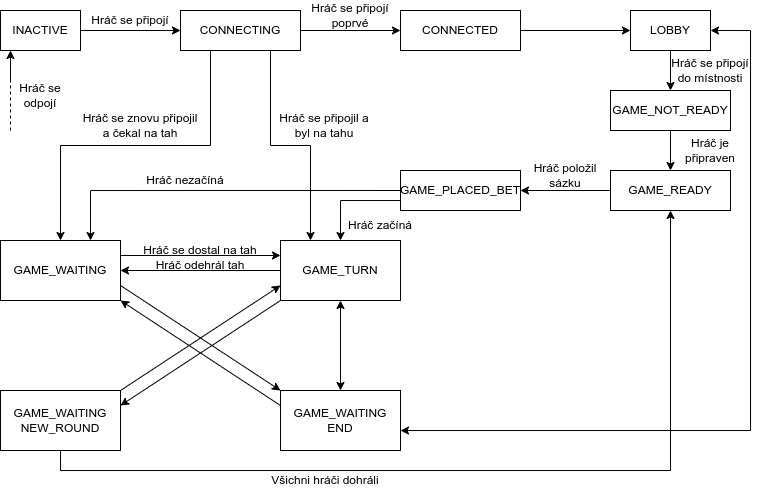
\includegraphics[width=0.8\textwidth]{stateDiagram.png}
\caption{Stavový diagram klienta}
\end{figure}

\newpage
Následující obrázek ilustruje přechody stavového diagramu klienta stejně jako předchozí, pouze značí, které příkazy převádějí diagram do kterých stavů. Některé stavy jsou měněny programem serveru a hráč jejich změnu neovlivní. Přechody ze všech stavů do stavu INACTIVE nejsou zakresleny kvůli přehlednosti stejně tak jako přechody činnostmi HIT a STAY mezi čtyřmi stavy rozehrané hry.

\begin{figure}[!htbp]
\centering
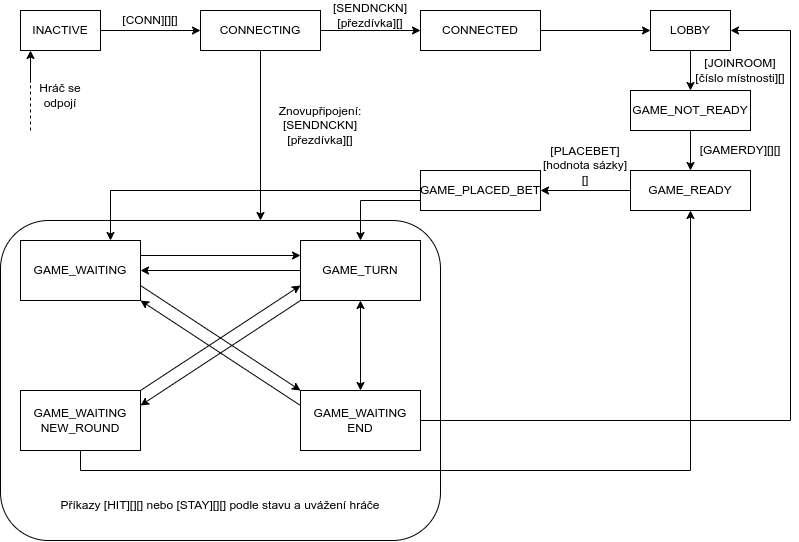
\includegraphics[width=0.8\textwidth]{stateDiagramCodes.png}
\caption{Stavový diagram klienta s kódy pro přechod}
\end{figure}

\subsection{Chybové stavy}

	Každá ze zpráv je zpracována tak, aby při správném průchodu vracela hodnotu 0. Pokud při zpracování nastane jakákoli chyba, vrátí příkaz zpracování nenulovou hodnotu podle čísla chyby. Tyto chybové stavy jsou zaznamenávány pro každého klienta a pokud počet chybných zpráv přesáhne danou hranici, hráč bude automaticky odpojen. Chybné stavy jsou vidět pouze na výstupu programu serveru, klientům tyto chybné stavy nejsou dostupné.
	
\newpage
\section{Implementace}
\subsection{Server}
Server je implementován v programovacím jazyce C. Program je rozdělen do následujících modulů:
\subsubsection{Card}
Tento modul obsahuje strukturu karty, která se používá ve hře. Uchovává hodnoty názvu karty a její hodnoty. 
\subsubsection{Client}
Tento modul obsahuje strukturu klienta a odpojeného klienta. Obě struktury jsou si velmi podobné, odpojený klient pouze nezahrnuje komunikační buffer a socket. Dále modul obsahuje funkce pro práci s klientem.
\subsubsection{ClientStates}
Tento modul obsahuje pouze výčet jednotlivých stavů klienta.
\subsubsection{Commands}
Tento modul obsahuje výčet příkazů, jejich název v protokolu a funkce, které tyto příkazy posílají danému klientovi.
\subsubsection{Game}
Tento modul je jeden z hlavních modulů programu. Obsahuje veškeré funkce pro manipulaci se všemi hrami a hráči. 
\subsubsection{Message}
Tento modul obsahuje strukturu zprávy, struktura obsahuje pouze řetězec o délce zprávy protokolu.
\subsubsection{Parser}
Tento modul obsluhuje přijaté zprávy a volá příslušné funkce programu.
\subsubsection{Queue}
Tento modul obsahuje implementaci fronty. Fronta byla v programu použita, aby se zamezilo ztrátě zpráv při použití příkazu select().
\subsubsection{Server}
Tento modul obsahuje funkce pro čtení a posílání dat, přečtená data dále předává modulu Parser.
\subsubsection{Signals}
Tento modul obsahuje obsluhu signálů programu, aby bylo možné server ukončit klávesovou zkratkou, nebo předáním signálu.
\subsubsection{StateMachine}
Tento modul obsahuje funkci pro obsluhu stavů klientů
\subsubsection{Stringop}
Tento modul obsahuje funkce pro práci s řetězci.

\subsection{Klient}
K vytvoření programu klienta byl využit herní engine Unity. Veškeré skriptování je implementováno v jazyce C\#. Implementace klienta je rozdělena do dvou hlavních tříd.
\subsubsection{NetworkDriver}
Tato třída obsluhuje síťový provoz mezi klientem a serverem. Poslouchání příchozích dat běží v odděleném vlákně, což vytváří problém při práci s UI klienta. Unity není ve většině případů thread-safe, proto přijaté zprávy po kontrole předává třída NetworkDriver třídě UIDRriver.
\subsubsection{UIDriver}
Tato třída se stará o veškerou manipulaci s UI. Zpracovává přijaté příkazy, které obdrží od třídy NetworkDriver ve frontě příkazů. Ty pak postupně zpracovává v hlavním vlákně programu

\subsection{Paralelismus}
Pro paralelní zpracování na straně serveru je použit příkaz select(). Ten umožňuje v jednom vlákně spravovat více připojení. Veškeré příchozí zprávy jsou zapsány do fronty, odkud jsou pak postupně vybírány a zpracovávány. Každá instance hry na serveru je uchovávána v jedné struktuře, její stav se mění v závislosti na příchozích zprávách. Každý klient má zapsanou hru, ve které hraje, podle té lze identifikovat, která instance hry bude ovlivněna. 

\newpage
\section{Požadavky na překlad}
\subsection{Server}

\subsection{Klient}
Spustitelný soubor klienta je zapotřebí sestavit v herním enginu Unity verze 2021.3 a výše. Spustitelný soubor se vygeneruje pomocí menu File-Build and run. Tato činnost sestaví aktuální verzi programu a spustí jej. Případné další možnosti se dají nastavit ve File-Build settings.

\subsection{Server}
K sestavení serveru je zapotřebí nástroje make a kompilátoru gcc verze 12.2.0 (GCC). Sestavení programu je provedeno zavoláním příkazu make v adresáři programu (Na úrovni složky src). Po zavolání příkazu make se v podsložce bin vytvoří spustitelný soubor serveru.

\newpage
\section{Závěr}
Nejvíce byla tato práce přínosná pro zdokonalení a hlubšímu pochopení programování v jazyce C, což považuji za velmi přínosné. Dále tato práce zdokonalila mé chápání síťového provozu a práce se sockety. Bylo pouze velmi stresující snažit se ošetřit veškeré chybné stavy tak, aby program běžel bez problémů, jelikož počet takovýchto stavů není nejmenší. 
\end{document}